\documentclass{article}
\usepackage[utf8]{inputenc}
\usepackage[margin=1in]{geometry}
\usepackage{fancyhdr, parskip, wrapfig, hyperref, apacite, graphicx, setspace, multicol, bm}

\hypersetup{
    colorlinks = true,
    linkcolor = black,
    citecolor = black,
    urlcolor = black
}

\newenvironment{Figure}
  {\par\medskip\noindent\minipage{\linewidth}}
  {\endminipage\par\medskip}

\bibliographystyle{apacite}

\newcommand*\pct{\scalebox{.85}{\%}}

\pagestyle{fancy}
\lhead{STAT 225 Journal Assignment 1}
\rhead{M. C. Gîrjău, B. Wang}

\title{\Huge STAT 225 Journal Assignment 1 \\
\Large ``A Comparison of Artificial Incubation and Natural Incubation Hatching Success of Gopher Tortoise Eggs In Southern Mississippi''}
\author{\Large Maria-Cristiana Gîrjău, Brandon Wang}

\begin{document}
\maketitle

% The nonparametric methods can either be correctly or incorrectly applied.Write a brief summary of the article, including the research question, the specific hypotheses of the test, and the results of the analysis. If you believe the nonparametric method was correctly used, write a justification of why the analysis was appropriate. If you believe the nonparametric method was incorrectly used, write a critique of the application, including a more appropriate data analysis.Please be aware that part of this assignment is practicing your communication skills.  This should be a formally written document with minimal grammatical and spelling errors and proper citation of sources.

% \doublespacing

\begin{multicols}{2}

\subsection*{Introduction}

The Gopher Tortoise (\textit{Gopherus polyphemus}) is the only native North American tortoise species east of the Mississippi River. Gopher Tortoise numbers have been declining drastically in recent years, particularly in the western portion of their territory. This has led the state of Mississippi to officially categorize the species as ``endangered''. As part of a federal recovery plan, studies were conducted in order to uncover the causes of the Gopher Tortoise population decline. Previous research suggests that low recruitment is largely to blame, specifically low hatching success rates for their eggs, even when nests are protected from predators.

The article \textit{``A Comparison of Artificial Incubation and Natural Incubation Hatching Success of Gopher Tortoise Eggs In Southern Mississippi''} \cite{source} attempts to dig deeper into the reasons for the Gopher Tortoise population decline, investigating whether these observed low hatching success rates are due to reduced egg quality or underlying health issues (intrinsic factors), unsuitable nest environments resulting from habitat degradation (extrinsic factors), or a combination thereof.

\begin{Figure}
    \centering
    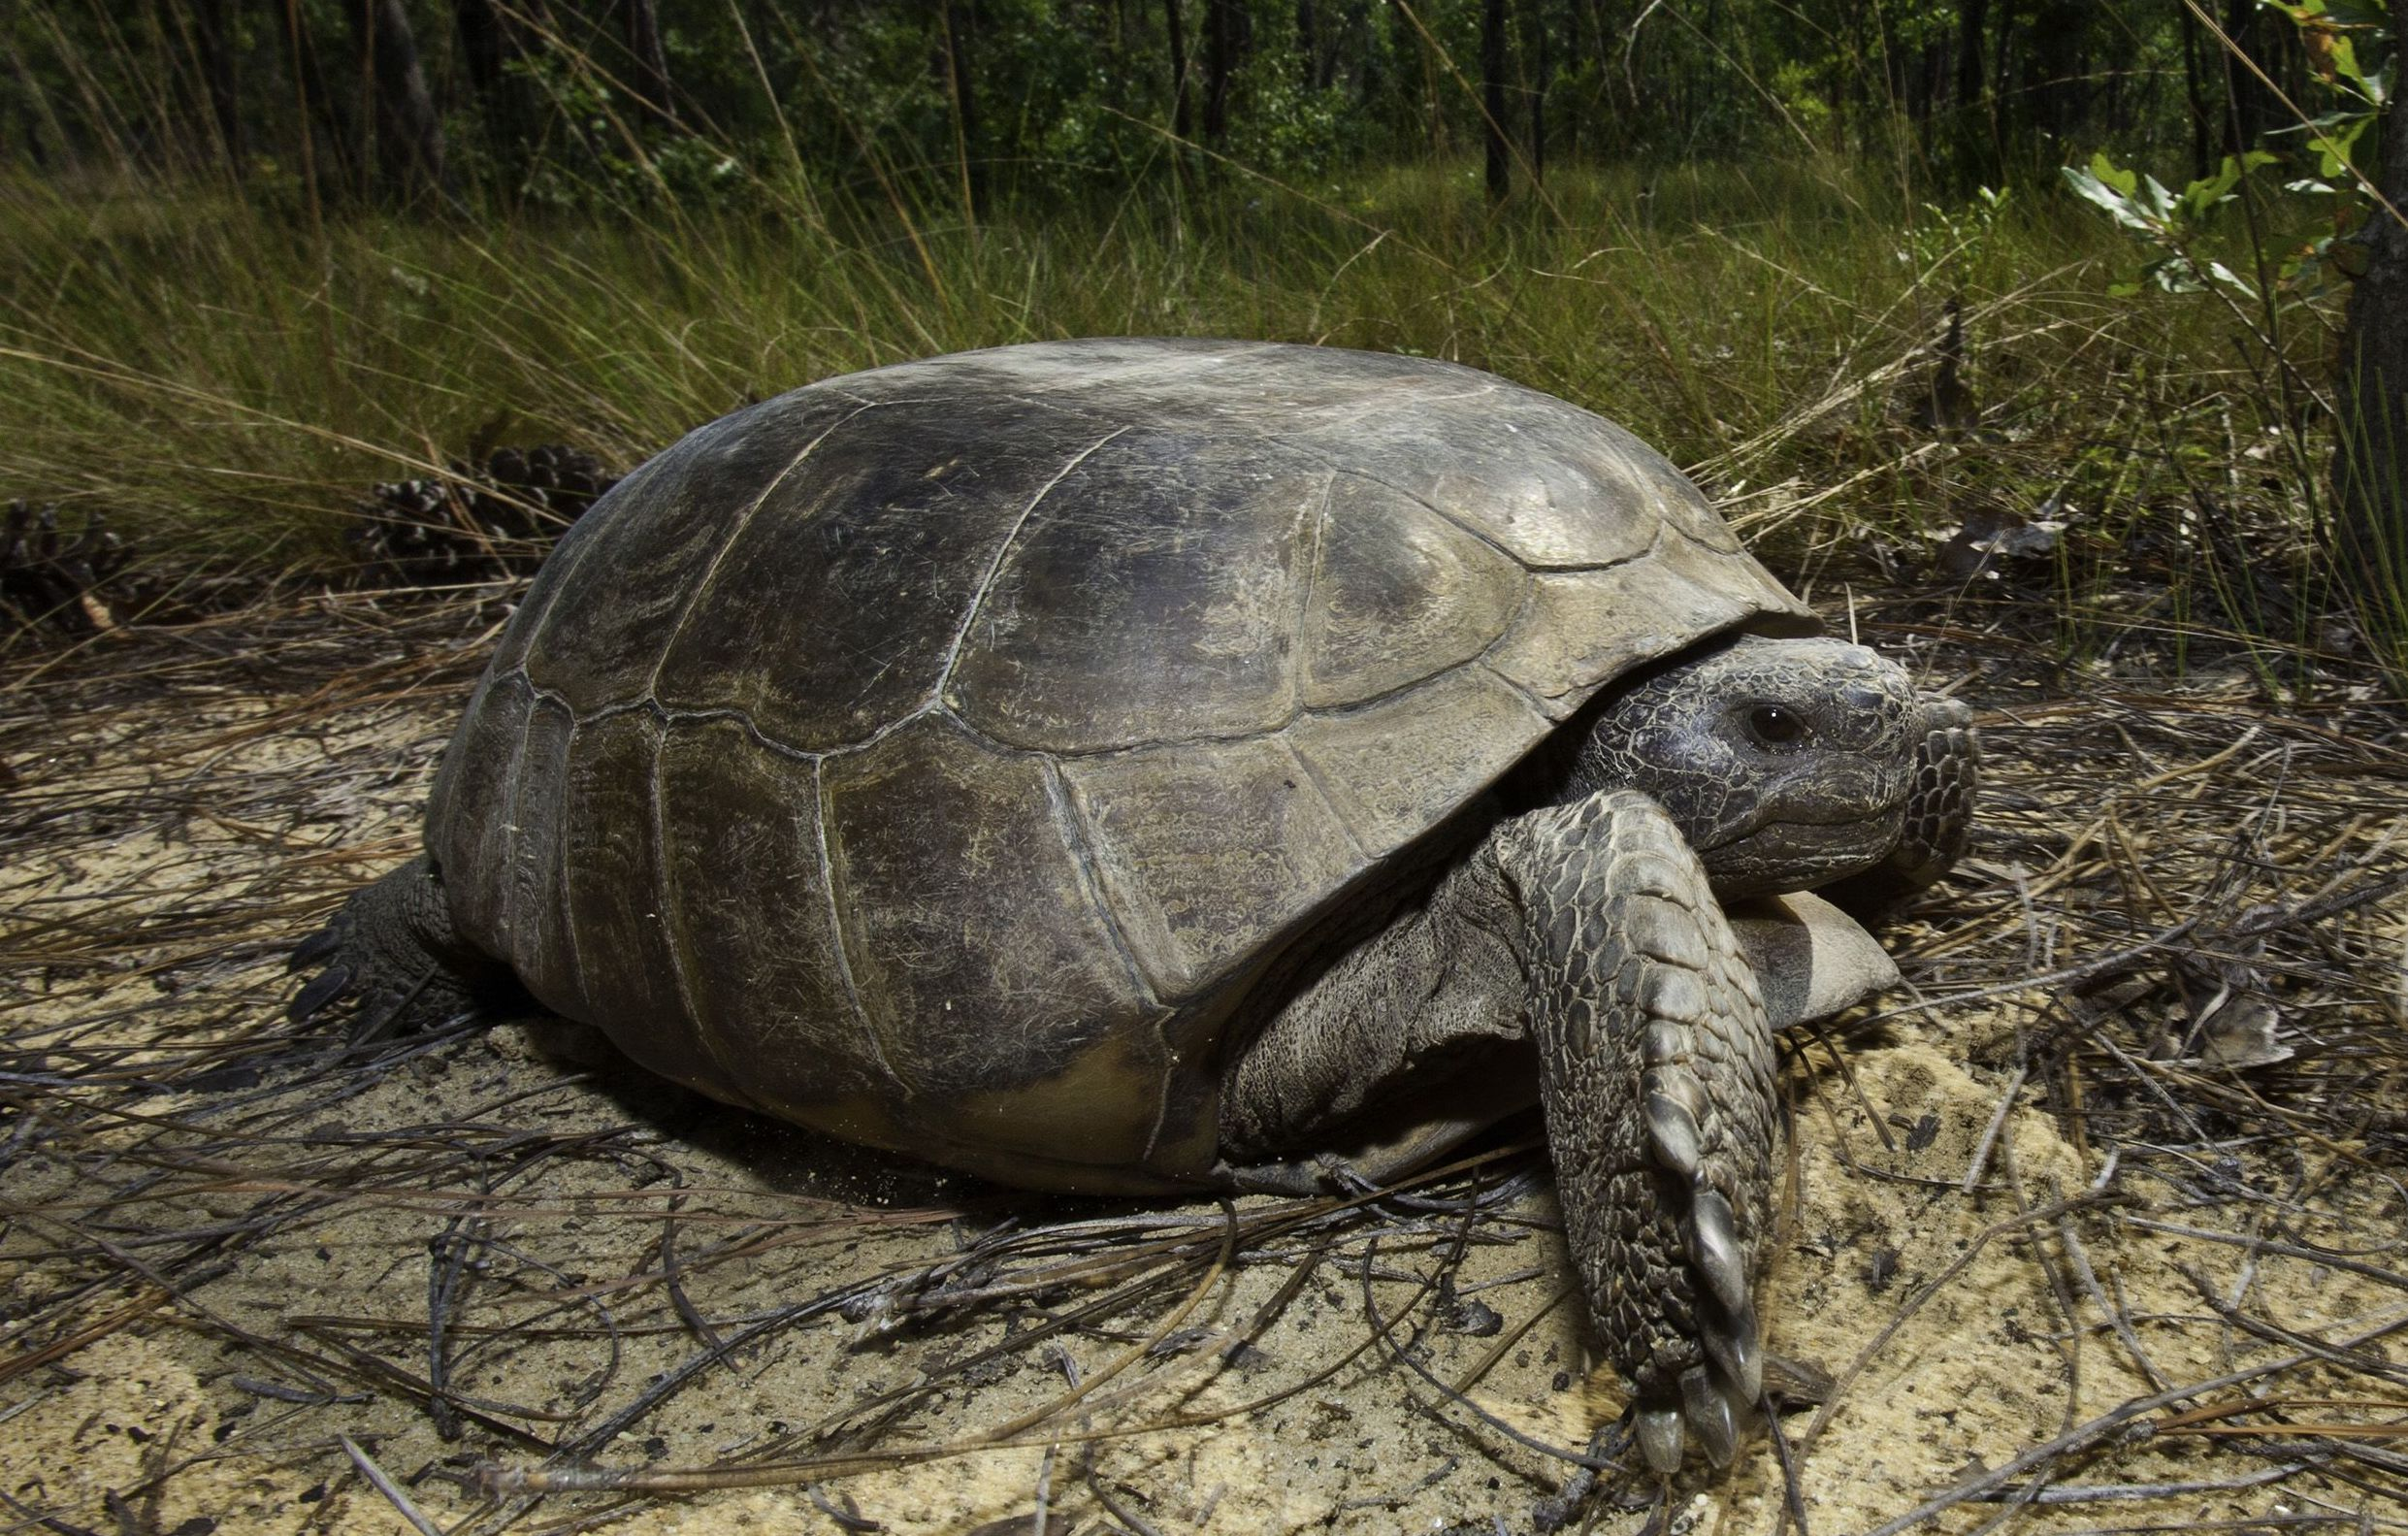
\includegraphics[width=0.95\linewidth]{tortoise.jpg}
    Figure 1 - A Mississippi Gopher Tortoise \\ \cite{pic}
\end{Figure}

\subsection*{Methodology}

The researchers identified a number of different Gopher Tortoise nests within an actively managed reserve, and carefully excavated all eggs from each nest, noting their original positions in order to put them back with minimal disturbance. Each egg was measured, weighed, and visually inspected to check for evidence of a live embryo, thus ensuring theoretical viability. On average, each Gopher Tortoise clutch (i.e. collection of eggs from the same nest) contains around 5 eggs, so two eggs were randomly chosen for artificial incubation, and all remaining eggs were put back in their original nests, in the exact same location they were found. 

All natural nests were protected against predators, and monitored twice weekly. The eggs intended for artificial incubation were taken to a laboratory and placed in optimal hatching conditions (as determined by previous research). The natural incubation period of the Gopher Tortoise ranges between 80 and 110 days, so both sets of eggs were inspected after a generous 127 days, to ensure all embryos have either successfully hatched or died. 

The researchers identified 17 nests, containing 87 eggs in total - 53 of these were incubated in the field, and 34 in the laboratory. Hatching success (as a percentage) was then calculated for each nest's naturally and artificially incubated complements, and the difference between them was computed. The final dataset then consisted of $n = 17$ difference measurements, with one observation per nest.

Since appropriate normality conditions did not hold for these measurements, the researchers decided to conduct a nonparametric matched-pairs Wilcoxon Signed Rank Test in order to investigate whether artificially incubated eggs have significantly higher hatching success rates than their counterparts in the wild. 


\newpage
\subsection*{Data Analysis}

The researchers hypothesized that eggs placed in the incubator will have significantly higher hatching success rates than the eggs left in their natural habitat. Letting $\theta = p_1 - p_2$ be the pairwise per-nest difference between $p_1$, the proportion of artificially incubated eggs that hatched successfully, and $p_2$, the proportion of eggs from the same clutch that hatched successfully in the field, we have our test hypotheses:
$$H_0: \theta \leq 0$$
$$H_A: \theta > 0$$

A matched-pairs Wilcoxon Signed Rank Test conducted at a significance level of $\alpha = 0.05$ confirmed the researchers' suspicions - hatching success for artificially incubated eggs was indeed significantly higher than that of related eggs incubated in the wild ($W_{16} = 35.0, p = 0.003 < 0.05$).

\subsection*{Results}

Mean hatching success rate for laboratory-incubated eggs was $58.8 \pm 44.14\pct$, with 22 eggs producing healthy tortoise hatchlings. In comparison, only $16.7 \pm 27.64\pct$ of eggs incubated in the field hatched successfully, thus yielding a mean pairwise difference of $42.1\pct$ between the two egg sets from a typical nest.

\subsection*{Conclusions}

The study concludes that both intrinsic and extrinsic factors play a role in the low hatching success rates of Gopher Tortoise eggs. The effect of \textit{extrinsic} factors on hatching success, such as environmental conditions or habitat degradation, can be quantified as the aforementioned $42.1\pct$ average difference between artificially incubated eggs and those incubated in the field. Similarly, since the mean success rate for optimal incubation was $58.8\pct$, the remaining $100\pct - 58.8\pct = 41.2\pct$ of eggs should theoretically have been able to hatch, but failed due to \textit{intrinsic} factors, such as poor egg quality or embryo health. 

\subsection*{Critique}

The article seems to have applied the nonparametric procedure appropriately. Supplied with inherently paired data (i.e. eggs of a similar provenance assigned to two experimental treatments), a one-sided upper-tailed matched-pairs Wilcoxon Signed Rank Test was used to test whether a statistic $\theta$ (here, the difference in hatching success rates $\theta = p_1 - p_2$) is statistically significantly greater than some hyothesized measure of location (here, $\theta_0 = 0$ under the null). 

While the article doesn't explicitly check the assumptions of the Signed Rank Test, they are mostly reasonable (items 1-3), with one exception (item 4):
\begin{enumerate}
    \itemsep-0.3em
    \item The data is \textbf{inherently paired} (by virtue of the experimental design) and drawn \textbf{from the same population} of Gopher Tortoises;
    \item The nests are randomly sampled to ensure \textbf{independence} between pairwise nest differences;
    \item Hatching success rates (specifically, proportions) are both \textbf{continuous} and \textbf{ordinal};
    \item The pairwise nest differences are assumed to be \textbf{symmetrically distributed with median $\boldsymbol{\theta_0 = 0}$} under the null hypothesis. The article makes no mention of this at all.
\end{enumerate}

Another point of contention is whether the Signed Rank Test is the best choice for this analysis. Since the sample sizes $n_i$ (based on which proportions are computed) differ by clutch, a more appropriate test would probably be a Permutation Test in which the eggs from each of the 17 clutches are randomly split between lab and field, and the difference in their hatching success rates is computed a large number of times. This way, laxer assumptions need to hold, and there would be no potential issues with tied data.

Overall, the article provides a good illustration of the paired Wilcoxon Signed Rank Test applied to a biological experiment. The study draws statistically appropriate conclusions, rejecting the null at a 0.05 significance level - there are indeed significant differences in the hatching success rates of related eggs under natural and artificial incubation conditions. 

\end{multicols}

\bibliography{references}

\end{document}